\chapter{Graph}

\section{Basic}
\runinhead{Graph representation.} $V$ for a vertex set with a map, mapping from vertex to its neighbors. The mapping relationship represents the edges $E$.
\begin{python}
V = defaultdict(list)
\end{python}

\runinhead{Complexity.} Basic complexities:

\begin{tabular}{lll}
\hline\noalign{\smallskip}
\textbf{Algorithm} & \textbf{Time}  & \textbf{Space}\\
\noalign{\smallskip}\hline\noalign{\smallskip}
dfs & $O(|E|)$ & $O(|V|), O(\text{longest path})$ \\
bfs & $O(|E|)$ & $O(|V|)$ \\
\noalign{\smallskip}\hline\noalign{\smallskip}
\caption{CAPTIONS}
\end{tabular}

\runinhead{Graph \& Tree.} For a undirected graph to be a tree, it needs to satisfied two conditions:
\begin{enumerate}
\item Acyclic
\item All connected
\end{enumerate}
\section{DFS}
\rih{Number of Islands.} The most fundamental and classical problem.
\begin{python}
11000
11000
00100
00011
Answer: 3
\end{python}
\rih{Clue}:
\begin{enumerate}
\item Iterative dfs
\end{enumerate}
\begin{python}
class Solution(object):
  def __init__(self):
    self.dirs = [(-1, 0), (1, 0), (0, -1), (0, 1)]

  def numIslands(self, grid):
    cnt = 0
    visited = [[False for _ in xrange(n)]
               for _ in xrange(m)]
    for i in xrange(m):
      for j in xrange(n):
        if not visited[i][j] and grid[i][j] == "1":
          self.dfs(grid, i, j, visited)
          cnt += 1

    return cnt
\end{python}

\begin{python}
  def dfs(self, grid, i, j, visited):
    m = len(grid)
    n = len(grid[0])
    visited[i][j] = True

    for dir in self.dirs:
      I = i+dir[0]
      J = j+dir[1]
      if (0 <= I < m and 0 <= J < n and
        not visited[I][J] and grid[I][J] == "1"):
        self.dfs(grid, I, J, visited)
\end{python}
If the islands are constantly updating and the query for number of islands is called multiple times, need to use union-find (Section \ref{section:unionFind}) to reduce each query's complexity from $O(mn)$ to $O(\log mn)$.

\section{BFS}
\subsection{BFS with Abstract Level}
Start bfs with a set of vertices in abstract level, not necessarily neighboring vertices.

Example: $-1$ obstacles, $0$ targets, calculate all other vertices' Manhattan distance to its nearest target:
$$
\begin{bmatrix}
\infty & -1 & 0 & \infty \\
\infty & \infty & \infty & -1 \\
\infty & -1 & \infty & -1 \\
0 & -1 & \infty & \infty \\
\end{bmatrix}
$$

is calculated as:
$$
\begin{bmatrix}
3 & -1 & 0 & 1 \\
2 & 2 & 1 & -1 \\
1 & -1 & 2 & -1 \\
0 & -1 & 3 & 4 \\
\end{bmatrix}
$$
\newpage
\rih{Code:}
\begin{python}
self.dirs = ((-1, 0), (1, 0), (0, -1), (0, 1))

def wallsAndGates(self, mat):
  q = [(i, j) for i, row in enumerate(mat)
     for j, val in enumerate(row) if val == 0]
  for i, j in q:  # iterator
    for d in self.dirs:
      I, J = i+d[0], j+d[1]
      if (0 <= I < m and  0 <= J < n and
        mat[I][J] > mat[i][j]+1):
        mat[I][J] = mat[i][j]+1
        q.append((I, J))
\end{python}


\section{Detect Acyclic}
\begin{enumerate}
\item \pythoninline{marked} is reset after a dfs.
\item \pythoninline{visited} should be updated only in the end of the dfs.
\item For directed graph:
\begin{enumerate}
\item Should dfs for all neighbors except for vertices in \pythoninline{visited}, to avoid revisiting. For example, avoid revisiting A, B when start from C in the graph $C \rightarrow A \rightarrow B$.
\item Excluding predecessor \pythoninline{pi} is erroneous in the case of $A \leftrightarrow B$
\end{enumerate}
\item For undirected graph:
\begin{enumerate}
\item Should dfs for all neighbors except for the predecessor \pythoninline{pi}. $A-B$.
\item Excluding neighbors in \pythoninline{visited} is redundant, due to \pyinline{pi}.
\end{enumerate}
\end{enumerate}

\subsection{Directed Graph}
Detect cycles (any) in directed graph.

\begin{python}
def dfs(self, V, v, visited, pathset):
  if v in pathset:
    return False

  pathset.add(v)
  for nbr in V[v]:
    if nbr not in visited:
      if not self.dfs(V, nbr, visited, pathset):
        return False

  pathset.remove(v)
  visited.add(v)
  return True
\end{python}


\subsection{Undirected Graph}
Detect cycles (any) in undirected graph.

\begin{python}
def dfs(self, V, v, pi, visited, pathset):
  if v in pathset:
    return False

  pathset.add(v)
  for nbr in V[v]:
    if nbr != pi:
      if not self.dfs(V, nbr, v, visited, pathset):
        return False

  pathset.remove(v)
  visited.add(v)
  return True
\end{python}

\section{Topological Sorting}
For a graph $G=\{V, E\}$, if $A \rightarrow B $, then $A$ is before $B$ in the ordered list.
\subsection{Algorithm}
\rih{Core clues}:
\begin{enumerate}
\item \textbf{Dfs neighbors first}. If the neighbors of current node is  $\neg$visited, then dfs the neighbors
\item \textbf{Process current node}. After visiting all the neighbors, then visit the current node and push it to the result queue.

\end{enumerate}
Notice:
\begin{enumerate}
\item Need to check ascending order or descending order.
\item Need to \textbf{detect cycle}; thus the dfs need to construct result queue and detect cycle simultaneously, by using two sets: $visited$ and $pathset$.
\end{enumerate}
\newpage
\begin{python}
from collections import deque

def topological_sort(self, V):
  visited = set()
  ret = deque()

  for v in V.keys():
    if v not in visited:
      if not self.dfs_topo(V, v, visited, set(), ret):
        return []  # contains cycle

  return list(ret)

def dfs_topo(self, V, v, visited, pathset, ret):
  if v in pathset:
    return False

  pathset.add(v)
  for nbr in V[v]:
    if nbr not in visited:
      if not self.dfs_topo(V, nbr, visited, pathset, ret):
        return False

  pathset.remove(v)
  visited.add(v)
  ret.appendleft(v)
  return True

\end{python}

\subsection{Applications}
\begin{enumerate}
\item Course scheduling problem with pre-requisite.
\end{enumerate}

\section{Union-Find}\label{section:unionFind}
Improvements:
\begin{enumerate}
\item Weighting: size-baladnced tree
\item Path Compression.
\end{enumerate}}
\subsection{Algorithm}
Weighted union-find with path compression.\\
\rih{Core clues.}
\begin{enumerate}
\item \textbf{$\pi$ array}:an array to store each item's predecessor pi. The predecessor are lazily updated to its ancestor. When \pyinline{x == pi[x]}, then \pyinline{x} is the ancestor (i.e. root).
\item \textbf{Size-balanced}: merge the tree according to the size to maintain balance.
\item \textbf{Path compression}: Make the ptr in $\pi$ array to point to its root rather than its immediate parent.
\end{enumerate}
\begin{figure}[]
\centering
\subfloat{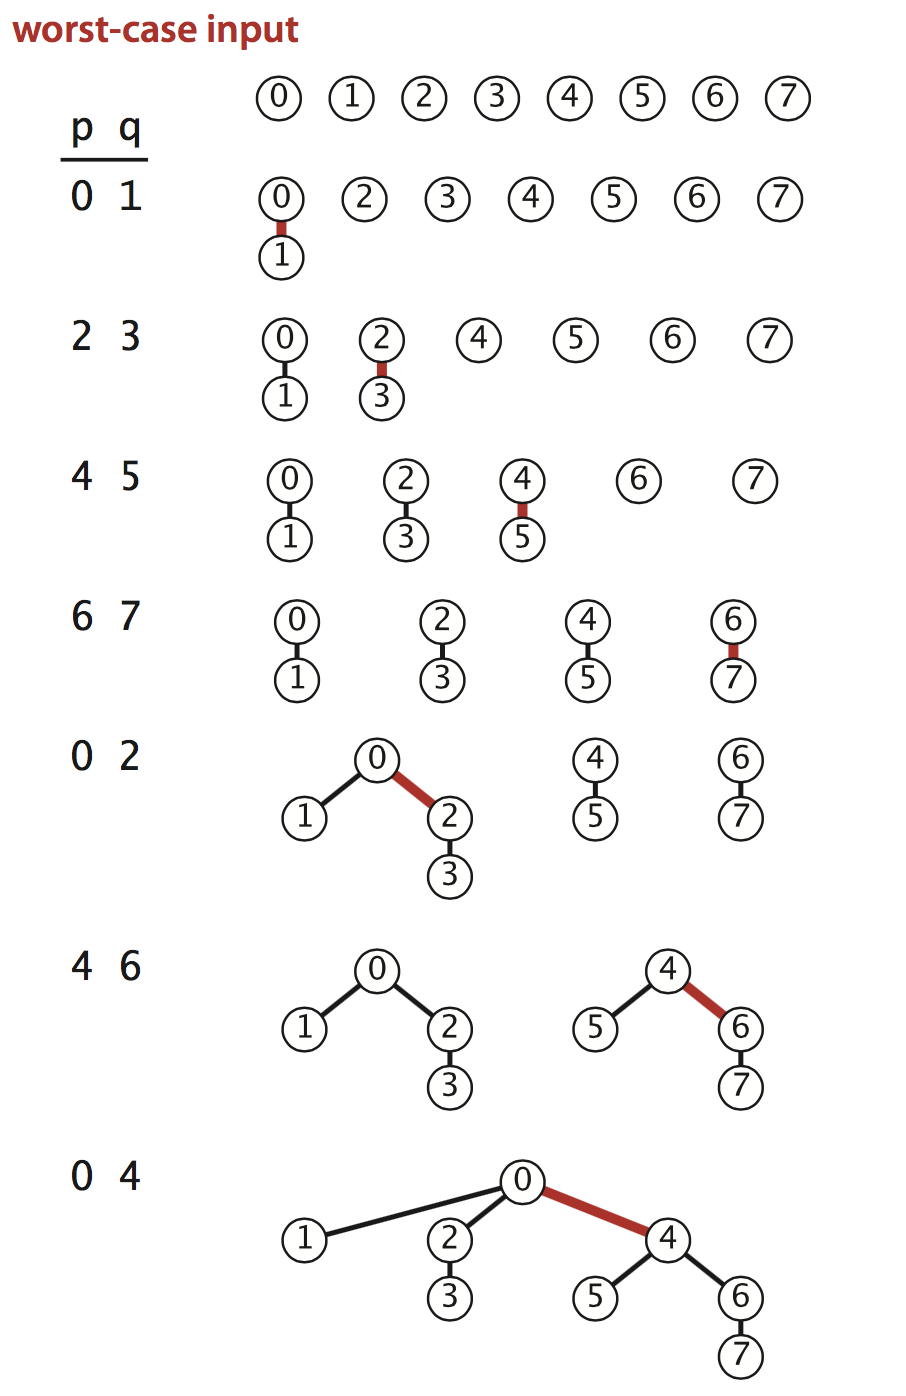
\includegraphics[scale=.70]{uf}}
\caption{Weighted quick-union traces}
\label{fig:union_find}
\end{figure}

\newpage
\begin{python}
class UnionFind(object):
  def __init__(self):
    self.pi = {}  # item -> pi
    self.sz = {}  # root -> size

  def __len__(self):
    """number of unions"""
    return len(self.sz)  # only root nodes have size

  def add(self, x):
    if x not in self.pi:
      self.pi[x] = x
      self.sz[x] = 1

  def root(self, x):
    """path compression"""
    pi = self.pi[x]
    if x != pi:
      self.pi[x] = self.root(pi)
    return self.pi[x]

  def unionize(self, x, y):
    pi1 = self.root(x)
    pi2 = self.root(y)

    if pi1 != pi2:
      if self.sz[pi1] > self.sz[pi2]:
        pi1, pi2 = pi2, pi1
        # size balancing
      self.pi[pi1] = pi2
      self.sz[pi2] += self.sz[pi1]
      del self.sz[pi1]

  def isunion(self, x, y):
    if x not in self.pi or y not in self.pi:
      return False
    return self.root(x) == self.root(y)
\end{python}

\subsection{Complexity}
$m$ union-find with $n$ objects: $O(n)+m O(\lg n)$


\section{Axis Projection}
Project the mat dimension from 2D to 1D, using \textit{orthogonal axis}.

\runinhead{Smallest bounding box.} Given the location $(x, y)$ of one of the 1's, return the area of the smallest bounding box that encloses 1's.
$$
\begin{bmatrix}
0& 0& 1& 0 \\
0& 1& 1& 0 \\
0& 1& 0& 0 \\
\end{bmatrix}
$$

Clues:
\begin{enumerate}
\item Project the 1's onto x-axis, binary search for the left bound and right bound of the bounding box.
\item Do the same for y-axis.
\end{enumerate}

Time complexity: $O(m\log n + n \log m)$, where $O(m), O(n)$ is for projection complexity.
\section{MST}
Minimum spanning tree.
\subsection{Kruskal's algorithm}
\textbf{Core clues:}
\begin{enumerate}
\item Vertices $v \in V$ are divided into different sets
\item Extract min edges to unionize the sets
\item Terminates when $\forall v\in V$ are in the same set.
\end{enumerate}
\textbf{Code:}
\begin{python}[mathescape]
def kruskal(G):
  ret = []
  uf = UnionFound()
  for v in G.V:
    uf.add(v)

  G.E.sort()  # sort by weights
  for u, v in G.E:
    if not uf.isunion(u, v):
      A.append((u, v))
      uf.unionize(u, v)
\end{python}
Complexity: $O(|E|\log |E|)$.
